\newpage
\section{モデル生物の構成および筋構造}
本章では今回モデルにする甲殻類の蟹について,外骨格と内骨格の違いや本研究で重要となる筋構造など実際にズワイガニを解剖した知見なども基に述べる.
%%%%%%%%%%%%%%%%%%%%%%%%%%%%%%%%%%%%%%%%%%%%%%%%%%%%%%%%%
\subsection{外骨格}
内骨格と外骨格の筋肉の付着の仕方を簡易的に示したものを図\ref{fig:naigai}に示す.
我々人間などの脊椎動物の骨のように身体の内部にあり筋肉の付着点となり,身体を支持する骨格を内骨格という.
それに対して本研究で扱う外骨格は身体を外側から覆い,体を支持し,内部を保護しつつ,筋肉の付着点となる硬い構造のことで甲殻類の外殻などが当てはまる.
外骨格は外敵からの防御にも重要な役割を果たしている反面,硬くて重い外骨格は身体の屈曲性や可動性を阻害することが多いが,甲殻類,昆虫類などは外骨格に多数の関節を持つため運動性に優れている.
しかし身体は完全に外骨格で覆われており成長が妨げられるため定期的に脱皮を行うことで身体を大きくしている.
%%%%%%%%%%%%%%%%%%%%%%%%%%%%%%%%%%%%%%%%%%%%%%%%%%%%%%%%%
\subsection{使用したモデル生物}
本研究では外骨格を持つモデル生物として甲殻類の十脚目短尾下目ケセンガニ科のズワイガニを用いた.
理由として蟹の中でも入手しやすく,モデルサイズも大きく解剖時に内部構造等の確認や測定が比較的容易なためである.
日本海全域のほか,房総半島以北の太平洋岸の水深50-450 mに生息し,北太平洋北部(オホーツク海,ベーリング海,カムチャッカ半島沿岸,アラスカ),北大西洋北部(カナダ東部,グリーンランド)に広く分布している\cite{R000000004-I11140373}.
実際に解剖に使用したズワイガニを図\ref{fig:zuwai}に示す.
重量:570 g,図\ref{fig:zuwai}の状態での縦横の長さ:132-372 mmの個体である.
ボイル後,冷凍したものを冷蔵庫で1日かけ解凍し,常温の室内で解剖を行った.
解剖は右半分の歩脚と鋏脚を対象に行った.
表\ref{tab:1setu}~表\ref{tab:5kadou}に第1肢から第5肢までの脚の寸法および可動域について測定した結果を示す.
表内における関節の名称については,図\ref{fig:setu}を参照されたい.
なお,解剖したズワイガニはボイル後の個体なので関節の可動域に関しては生きている状態での可動域とは異なる可能性がある.
%%%%%%%%%%%%%%%%%%%%%%%%%%%%%%%%%%%%%%%%%%%%%%%%%%%%%%%%%
\begin{figure}[b]
    \begin{minipage}{0.49\hsize}
      \vspace{15mm}
      \centering
      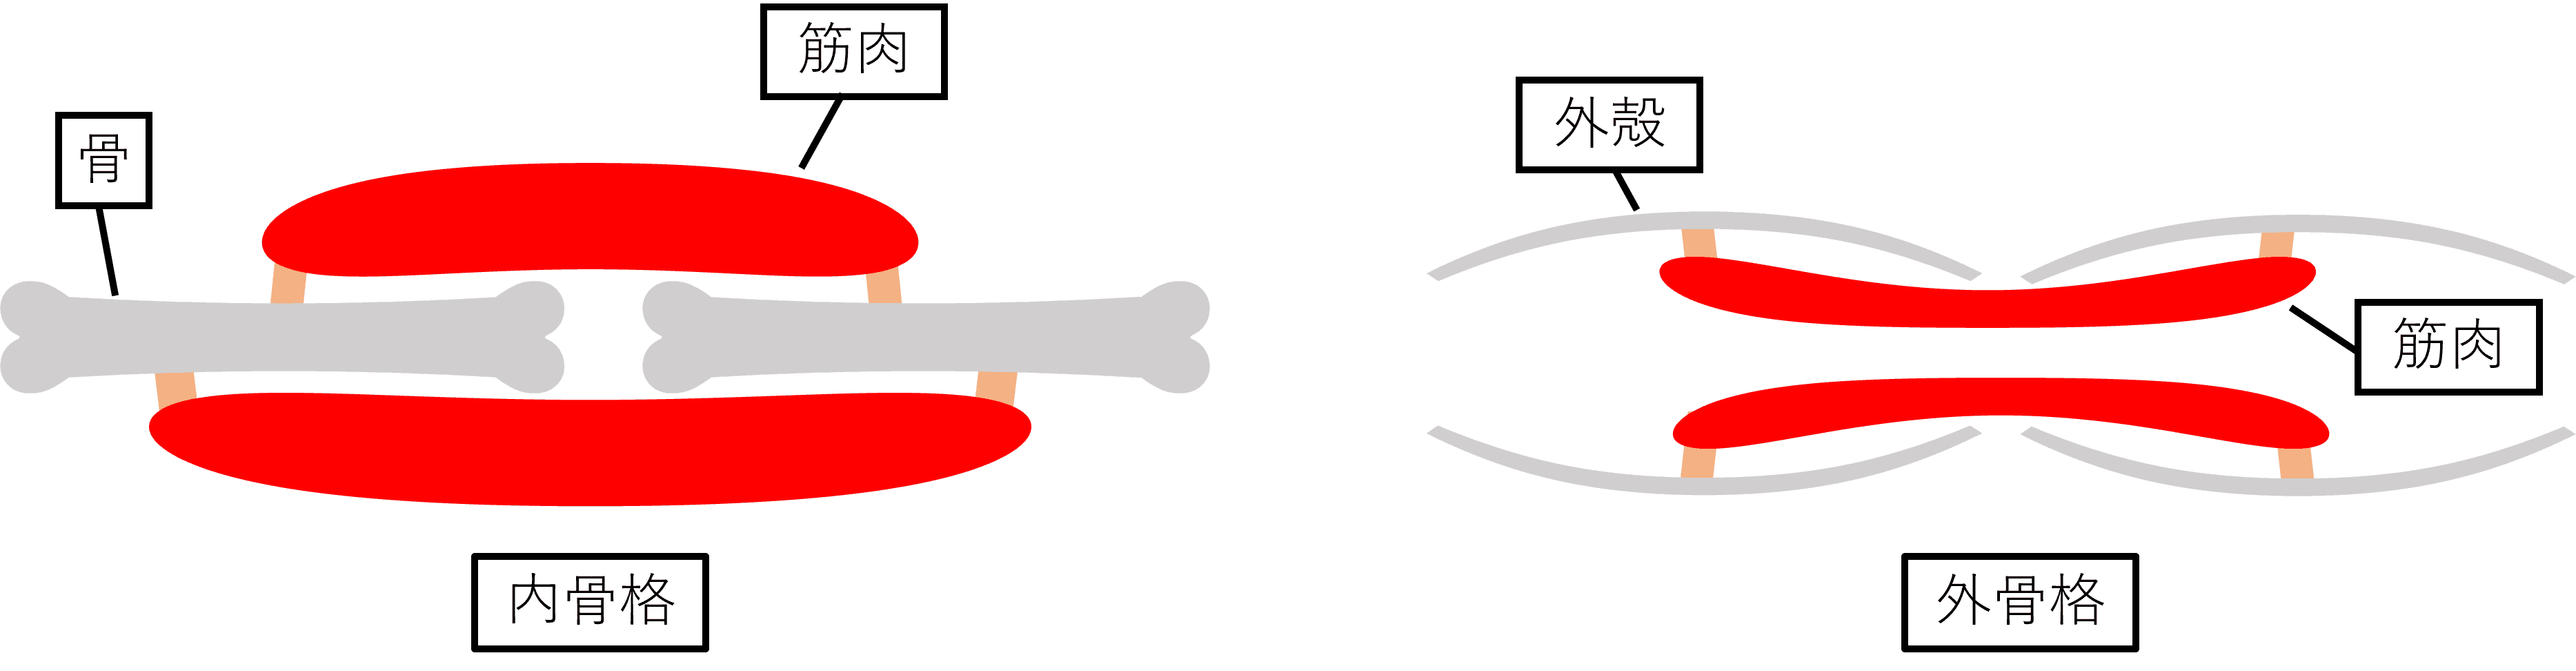
\includegraphics[scale=0.058]{image/kokkaku.png}
      \caption{内骨格と外骨格}
      \label{fig:naigai}
    \end{minipage}
    %
    \begin{minipage}{0.49\hsize}
      \centering
      \includegraphics[scale=.05]{image/apearance3_1.png}
      \caption{解剖に用いたズワイガニ}
      \label{fig:zuwai}
    \end{minipage}
\end{figure}
%%%%%%%%%%%%%%%%%%%%%%%%%%%%%%%%%%%%%%%%%%%%%%%%%%%%%%%%%
\begin{table}[htbp]
  \centering
  \caption{第1肢の長節から指節の寸法}
  \label{tab:1setu}
  \vspace{-3mm}
  \begin{tabular}{|l|c|c|c|c|c|}
  \hline
     & \multicolumn{1}{l|}{幅-左 [mm]} & \multicolumn{1}{l|}{幅-中 [mm]} & \multicolumn{1}{l|}{幅-右 [mm]} & \multicolumn{1}{l|}{厚み [mm]} & \multicolumn{1}{l|}{長さ [mm]} \\ \hline
  長節 & 12.01                       & 12.01                       & 8.86                        & 7.68                        & 52.0                        \\ \hline
  腕節 & 6.11                        & -                           & 9.85                        & 7.60                        & 14.5                        \\ \hline
  前節 & 10.39                       & -                           & 7.12                        & 4.26                        & 38.0                        \\ \hline
  指節 & -                           & 4.51                        & -                           & 3.36                        & 24.5                        \\ \hline
  \end{tabular}
\end{table}
%
\begin{table}[htbp]
  \centering
  \caption{第2肢の長節から指節の寸法}
  \label{tab:2setu}
  \vspace{-3mm}
  \begin{tabular}{|l|c|c|c|c|c|}
  \hline
     & \multicolumn{1}{l|}{幅-左 [mm]} & \multicolumn{1}{l|}{幅-中 [mm]} & \multicolumn{1}{l|}{幅-右 [mm]} & \multicolumn{1}{l|}{厚み [mm]} & \multicolumn{1}{l|}{長さ [mm]} \\ \hline
  長節 & 18.10                       & 19.05                       & 11.85                       & 9.18                        & 87.5                        \\ \hline
  腕節 & 8.59                        & -                           & 16.14                       & 7.32                        & 27.5                        \\ \hline
  前節 & 16.14                       & -                           & 8.83                        & 4.40                        & 58.5                        \\ \hline
  指節 & -                           & 5.43                        & -                           & 2.65                        & 25.0                        \\ \hline
  \end{tabular}
\end{table}
%
\begin{table}[htbp]
  \centering
  \caption{第3肢の長節から指節の寸法}
  \label{tab:3setu}
  \vspace{-3mm}
  \begin{tabular}{|l|c|c|c|c|c|}
  \hline
     & \multicolumn{1}{l|}{幅-左 [mm]} & \multicolumn{1}{l|}{幅-中 [mm]} & \multicolumn{1}{l|}{幅-右 [mm]} & \multicolumn{1}{l|}{厚み [mm]} & \multicolumn{1}{l|}{長さ [mm]} \\ \hline
  長節 & 18.38                       & 20.88                       & 13.56                       & 9.98                        & 102.0                       \\ \hline
  腕節 & 9.70                        & -                           & 17.30                       & 9.12                        & 31.5                        \\ \hline
  前節 & 17.06                       & -                           & 9.01                        & 4.91                        & 63.5                        \\ \hline
  指節 & -                           & 5.62                        & -                           & 3.93                        & 27.5                        \\ \hline
  \end{tabular}
\end{table}
%
\begin{table}[htbp]
  \centering
  \caption{第4肢の長節から指節の寸法}
  \label{tab:4setu}
  \vspace{-3mm}
  \begin{tabular}{|l|c|c|c|c|c|}
  \hline
     & \multicolumn{1}{l|}{幅-左 [mm]} & \multicolumn{1}{l|}{幅-中 [mm]} & \multicolumn{1}{l|}{幅-右 [mm]} & \multicolumn{1}{l|}{厚み [mm]} & \multicolumn{1}{l|}{長さ [mm]} \\ \hline
  長節 & 19.10                       & 21.74                       & 13.11                       & 11.05                       & 100.0                       \\ \hline
  腕節 & 10.57                       & -                           & 18.42                       & 8.74                        & 40.5                        \\ \hline
  前節 & 16.48                       & -                           & 10.40                       & 4.68                        & 70.0                        \\ \hline
  指節 & -                           & 5.60                        & -                           & 3.69                        & 30.0                        \\ \hline
  \end{tabular}
  \end{table}
  %
  \begin{table}[htbp]
    \centering
    \caption{第5肢(鋏脚)の長節から指節の寸法}
    \label{tab:5setu}
    \vspace{-3mm}
    \begin{tabular}{|c|c|c|c|}
    \hline
    \multicolumn{1}{|l|}{} & \multicolumn{1}{l|}{幅(左-中-右) {[}mm{]}} & \multicolumn{1}{l|}{厚み(左-中-右) {[}mm{]}} & \multicolumn{1}{l|}{長さ [mm]} \\ \hline
    長節                     & 18.10-18.23-18.24                     & 11.72-15.05-15.89                      & 63.5                        \\ \hline
    腕節                     & 11.70-18.40-19.31                     & 13.23-18.64-17.03                      & 15.5                        \\ \hline
    前節                     & 22.97-25.82-25.06                     & 14.75-21.30-19.09                      & 50.0                        \\ \hline
    前節(鋏部)                 & 8.64----                              & ----4.45                          & 45.0                      \\ \hline
    指節                     & 8.15----                              & ----4.26                               & 50.0                        \\ \hline
    \end{tabular}
  \end{table}
  %
  \begin{table}[htbp]
  \begin{minipage}{0.5\hsize}
    \centering
    \caption{第1肢の節間の可動域}
    \label{tab:1kadou}
    \vspace{-3mm}
    \begin{tabular}{|l|c|}
    \hline
       & \multicolumn{1}{l|}{可動域 [deg]} \\ \hline
    長節-腕節間 & 0-155                         \\ \hline
    腕節-前節間 & 0-81                          \\ \hline
    前節-指節間 & 0-110                         \\ \hline
    \end{tabular}
  \end{minipage}
  %
  \begin{minipage}{0.5\hsize}
    \centering
    \caption{第2肢の節間の可動域}
    \label{tab:2kadou}
    \vspace{-3mm}
    \begin{tabular}{|l|c|}
    \hline
       & \multicolumn{1}{l|}{可動域 [deg]} \\ \hline
    長節-腕節間 & 0-145                         \\ \hline
    腕節-前節間 & 0-50                          \\ \hline
    前節-指節間 & 0-90                          \\ \hline
    \end{tabular}
  \end{minipage}
  %
  \begin{minipage}{0.5\hsize}
    \centering
    \vspace{5mm}
    \caption{第3肢の節間の可動域}
    \label{tab:3kadou}
    \vspace{-3mm}
    \begin{tabular}{|l|c|}
    \hline
       & \multicolumn{1}{l|}{可動域 [deg]} \\ \hline
    長節-腕節間 & 0-150                         \\ \hline
    腕節-前節間 & 0-45                          \\ \hline
    前節-指節間 & 0-80                          \\ \hline
    \end{tabular}
  \end{minipage}
  %
  \begin{minipage}{0.5\hsize}
    \centering
    \vspace{5mm}
    \caption{第4肢の節間の可動域}
    \label{tab:4setukadou}
    \vspace{-3mm}
    \begin{tabular}{|l|c|}
    \hline
           & \multicolumn{1}{l|}{可動域 {[}deg{]}} \\ \hline
    長節-腕節間 & 0-140                            \\ \hline
    腕節-前節間 & 0-45                             \\ \hline
    前節-指節間 & 0-89                            \\ \hline
    \end{tabular}
  \end{minipage}
\end{table}
%
\begin{table}[htbp]
  \centering
  \vspace{5mm}
  \caption{第5肢の節間の可動域}
  \label{tab:5kadou}
  \vspace{-3mm}
  \begin{tabular}{|l|c|}
  \hline
         & \multicolumn{1}{l|}{可動域 [deg]} \\ \hline
  長節-腕節間 & 70-140                        \\ \hline
  腕節-前節間 & 0-40                          \\ \hline
  前節-指節間 & 15-30                         \\ \hline
  \end{tabular}
  \end{table}
%%%%%%%%%%%%%%%%%%%%%%%%%%%%%%%%%%%%%%%%%%%%%%%%%%%%%%%%%
\begin{figure}[t]
%
  \begin{minipage}{1\hsize}
    \centering
    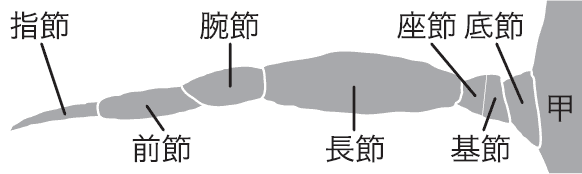
\includegraphics[scale=0.52]{image/setu.PNG}
    \caption{節の名称\cite{crabnature}}
    \vspace{3mm}
    \label{fig:setu}
  \end{minipage}
%
  \begin{minipage}{1\hsize}
    \centering
    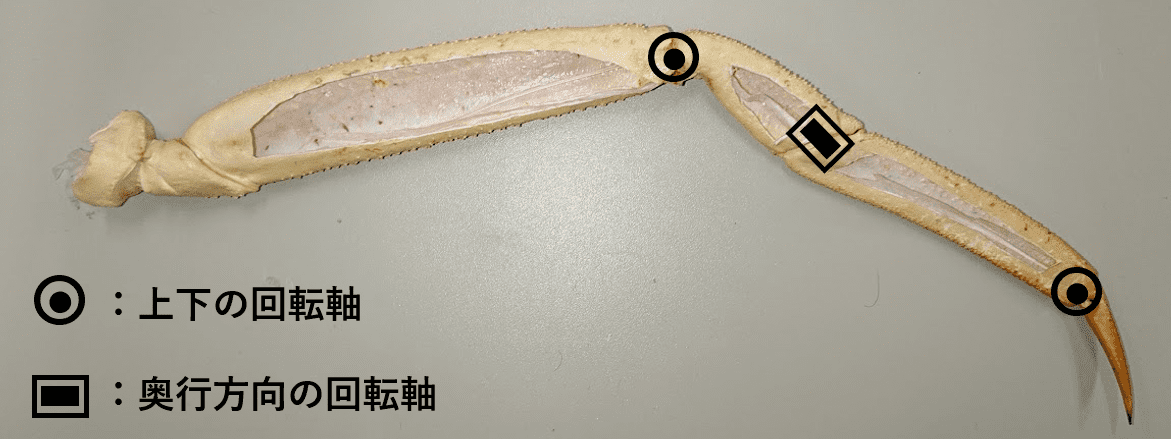
\includegraphics[scale=0.26]{image/kaiten.png}
    \caption{ズワイガニの脚の可動域}
    \label{fig:kaiten}
  \end{minipage}
  %
  \begin{minipage}{0.5\hsize}
    \centering
    \vspace{3mm}
    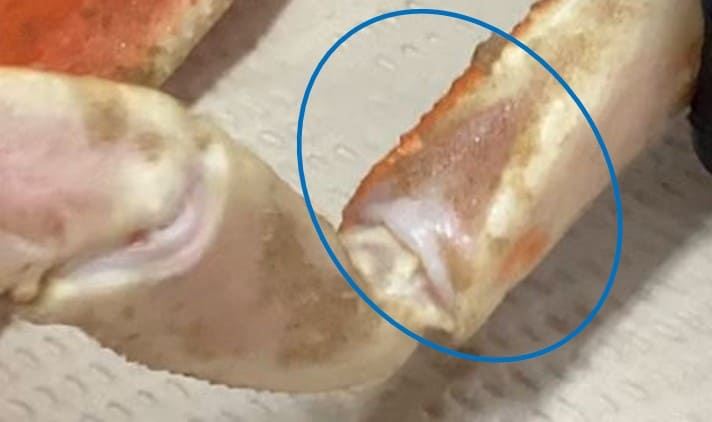
\includegraphics[scale=0.24]{image/maku1.JPG}
    \caption{節間膜}
    \label{fig:maku}
  \end{minipage}
%
    \begin{minipage}{0.5\hsize}
      \centering
      \vspace{4mm}
      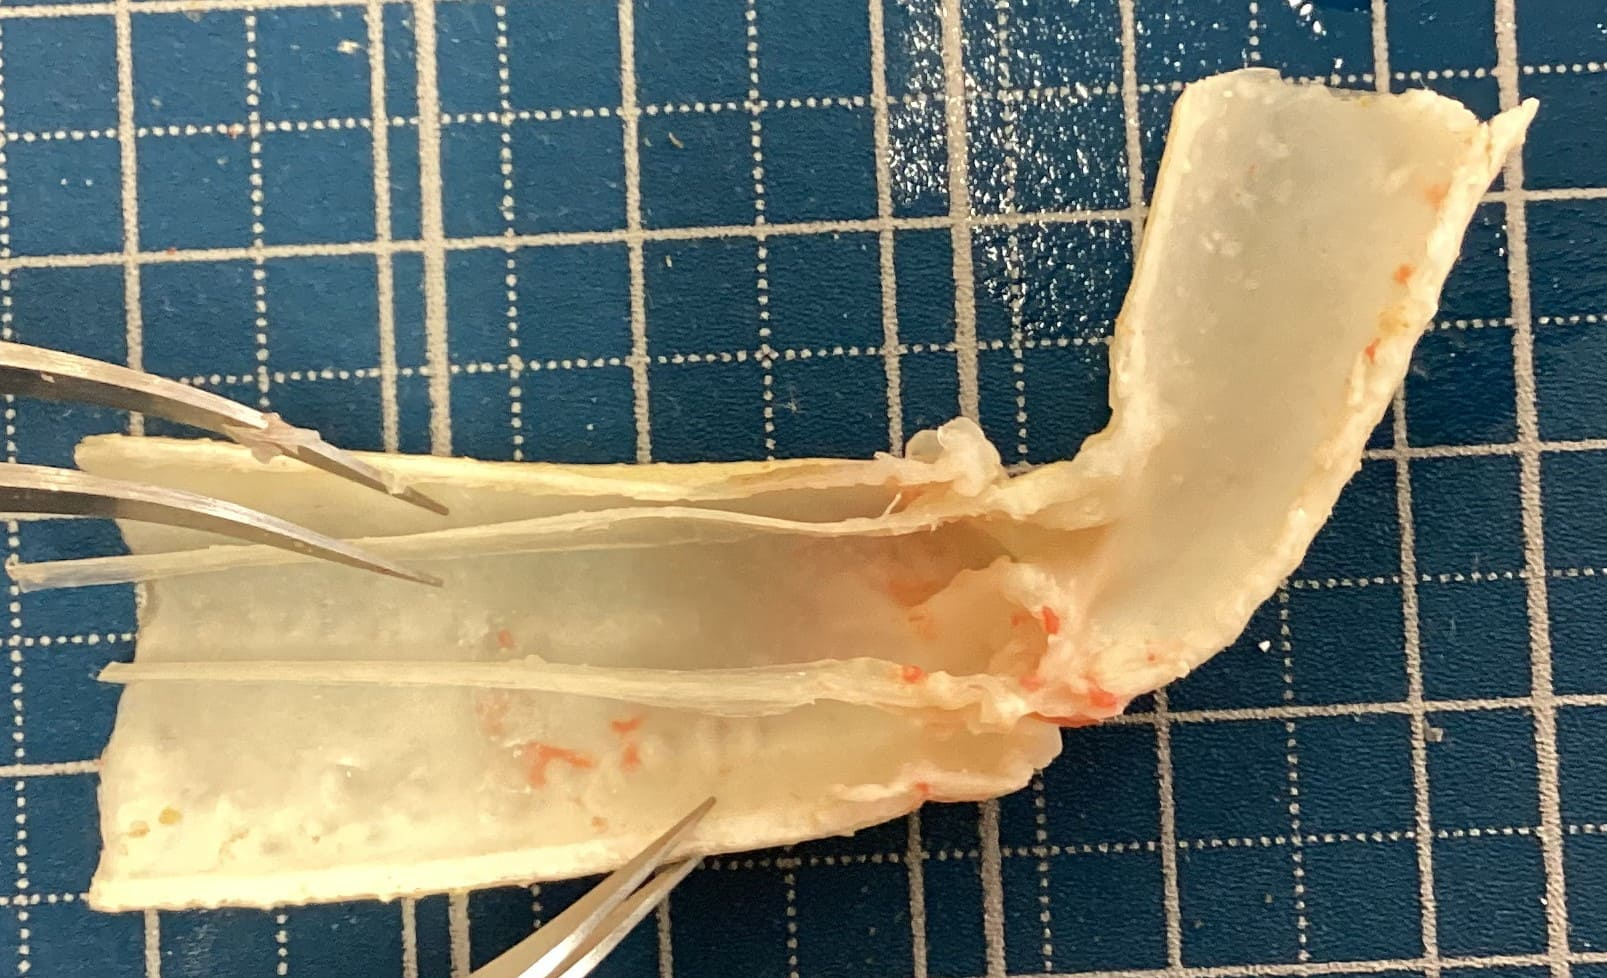
\includegraphics[scale=0.1]{image/setukanmaku.jpg}
      \caption{腱の様子}
      \label{fig:ken}
    \end{minipage}
  \end{figure}
%%%%%%%%%%%%%%%%%%%%%%%%%%%%%%%%%%%%%%%%%%%%%%%%%%%%%%%%%
\vspace{15mm}
\subsection{蟹の関節構造と筋構造および筋配置}
\subsubsection{関節構造}
蟹の脚は鋏脚と歩脚の5対10本から構成され,それぞれの脚は甲に近いほうから底節,基節,座節,長節,腕節,前節,指節の7つの節からなる(図\ref{fig:setu}).基節,座節の間の関節は融合し1つの節のように見える場合もある\cite{crabnature}.
脚を構成する7つの節が接する関節の部分はそれぞれ動く方向が決まっており,底節は複雑に配置された筋によって前後左右に動かすことが可能であるが,それよりも遠位の関節は基本的には単純な開閉動作をする.
図\ref{fig:kaiten}に解剖したズワイガニの歩脚に回転軸を追記したものを示す.
今回用いるズワイガニに関しては長節から指節のうち,腕節-前節間は前後に可動域を持つが,それ以外の節間は甲から腹側への開閉方向の可動域を持つことが分かった.
また,それぞれの節間には節間膜と呼ばれる丈夫で柔軟なクチクラ質の組織によって繋がっている(図\ref{fig:maku}).
%%%%%%%%%%%%%%%%%%%%%%%%%%%%%%%%%%%%%%%%%%%%%%%%%%%%%%%%%
\subsubsection{筋構造}
蟹の脚の筋肉について,蟹の脚内部を充填する筋繊維の一端は節の内壁に付着し,もう一方は腱と呼ばれる組織,いわゆる蟹のすじに付着する.
腱は隣の関節の端に繋がっており,筋繊維が収縮することによって腱が引っ張られ節が開閉する.
ズワイガニを解剖した際に記録した長節-腕節間の腱の様子を図\ref{fig:ken}に示す.
解剖結果よりズワイガニの腱は節間膜と一体になるように挿入されていることが分かった.
筋繊維は腱に対して斜めに充填されており,このように配置された筋繊維を羽状筋という.
羽状筋の動きの模式図を図\ref{fig:ujo}に示す.
羽状筋には2つの利点があるとされている.1つ目は収縮しても膨張せず,羽状筋の角度が大きくなるだけなので限られた狭い空間で働くのに適していること,2つ目は同じ形状と体積の平行筋と比べ収縮時に約2倍の力を発揮することが出来ることである\cite{warner1977biology}.
%%%%%%%%%%%%%%%%%%%%%%%%%%%%%%%%%%%%%%%%%%%%%%%%%%%%%%%%%
\subsubsection{筋配置}
脚内部の筋肉配置について,同じく十脚目短尾下目のLibinia emarginataの歩脚と鋏脚の筋構造を図\ref{fig:libinia}に,ヨーロッパイチョウガニとヨーロッパミドリガニの歩脚をCTスキャンしたものを図\ref{fig:ct}\subref{fig:ct1},\subref{fig:ct2}に示す.
図\ref{fig:libinia},図\ref{fig:ct}より,3種の歩脚の長節以降の筋配置は非常に似ていることが分かり,腕節-前節間,前節-指節間は節の可動域に沿って配置されているが,長節-腕節間は可動域よらず縦に配置されている.
また,図\ref{fig:libinia}より,底節,基節,座節部分は複雑な筋配置となっていることが分かる.
本研究ではズワイガニの長節-指節間の筋配置はこれらと同様なものとして扱い,節を開く方向に作用する羽状筋を開筋,閉じる方向へと作用するものを閉筋とする.
また,筋配置が複雑な底節,基節,座節は扱わないものとする.
%%%%%%%%%%%%%%%%%%%%%%%%%%%%%%%%%%%%%%%%%%%%%%%%%%%%%%%%%
\begin{figure}[t]
  \begin{minipage}{1\hsize}
    \centering
    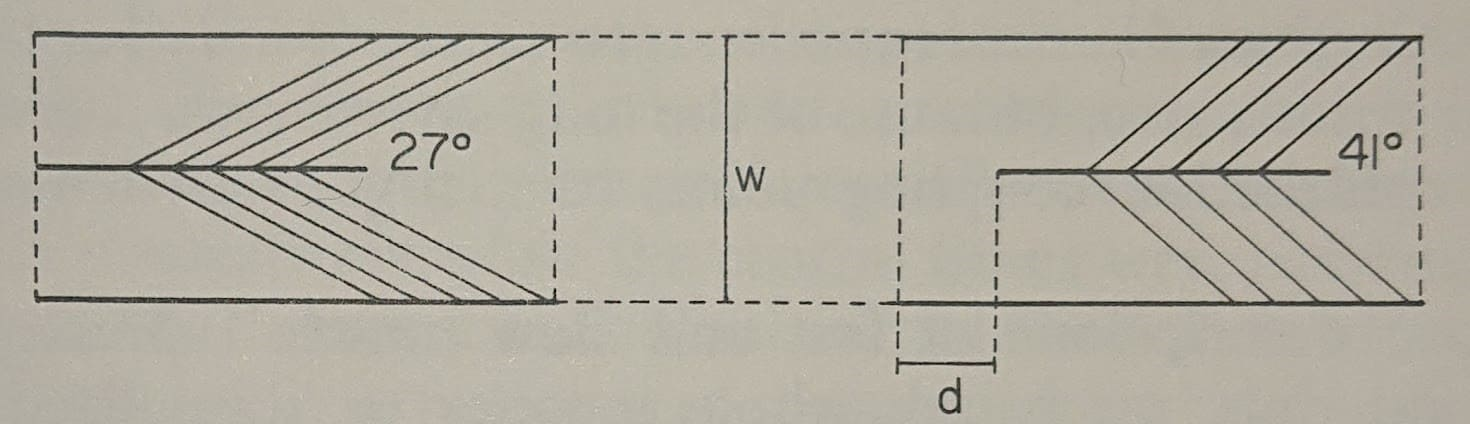
\includegraphics[scale=0.3]{image/ujo.JPG}
    \caption{羽状筋の動きを模式的に表したもの.左側が筋肉が伸展,右側が収縮した状態.収縮中,羽状筋の角度は27 degから41 degに増加し,腱は距離dを移動する.各筋繊維は短く太くなるが,筋全体の幅wは変化しない\cite{warner1977biology}}
   \label{fig:ujo}
  \end{minipage}
\end{figure}
  
\begin{figure}[t]
  \centering
  \vspace{-3mm}
  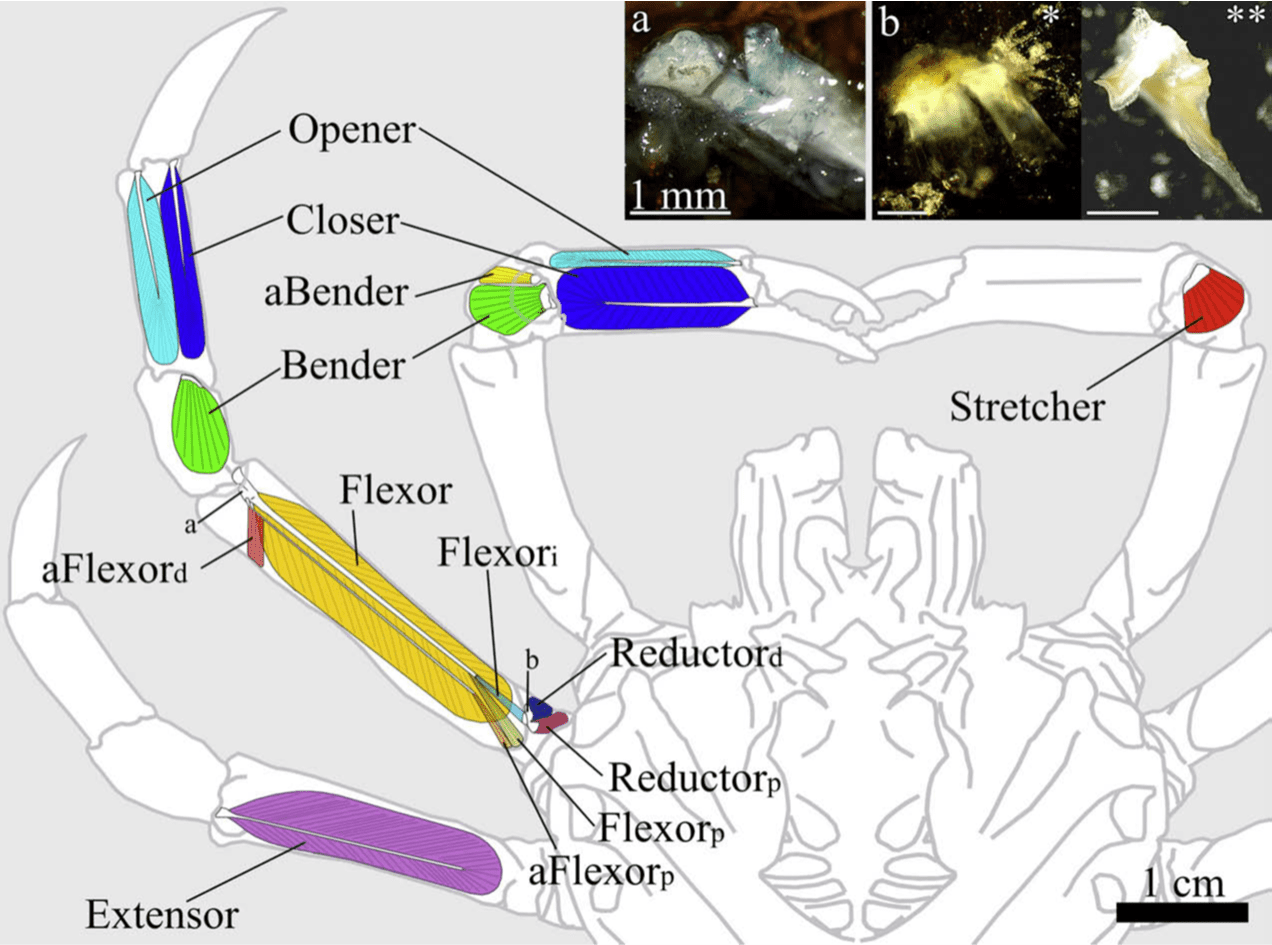
\includegraphics[scale=0.25]{image/libinia.png}
  \caption{Libinia emarginataの歩脚と鋏脚の筋構造\cite{VIDALGADEA2009179}}
  \label{fig:libinia}
\end{figure}
%
\begin{figure}[t]
%
  \begin{minipage}{0.45\hsize}
    \centering
    \vspace{5mm}
    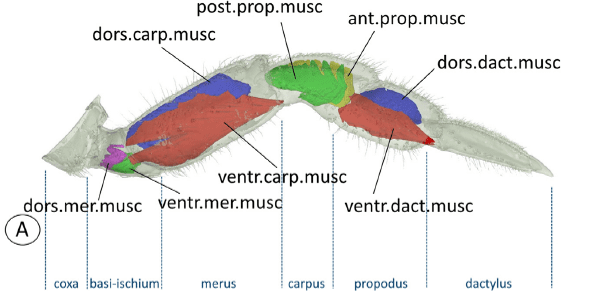
\includegraphics[scale=0.5]{image/crabct2.PNG}
    \subcaption{ヨーロッパイチョウガニ}
    % \vspace{3mm}
    \label{fig:ct1}
  \end{minipage}
  %
  \begin{minipage}{0.45\hsize}
    \centering
    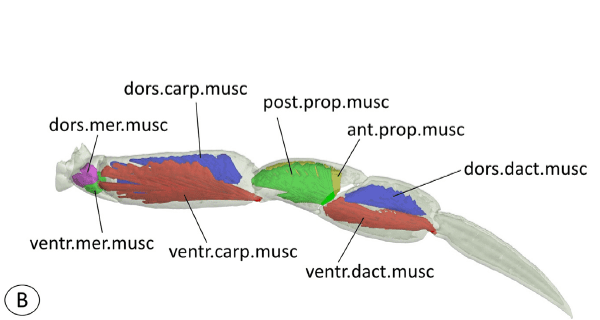
\includegraphics[scale=0.5]{image/crabct1.PNG}
    \subcaption{ヨーロッパミドリガニ}
    % \vspace{3mm}
    \label{fig:ct2}
  \end{minipage}
  \caption{歩脚のctスキャン画像\cite{HAZERLI2020100972}}
  \label{fig:ct}
%
\end{figure}
%%%%%%%%%%%%%%%%%%%%%%%%%%%%%%%%%%%%%%%%%%%%%%%%%%%%%%%%%





